%\documentclass[xetex,mathserif,serif]{beamer}
\documentclass{beamer}
\renewcommand{\tiny}{\fontsize{4}{14}\selectfont}

\usepackage{hyperref}
\usepackage{fontspec} 
\usepackage{xunicode} %Unicode extras!
\usepackage{xltxtra} %Fixes 
\usefonttheme{professionalfonts}
\setmainfont{Linux Libertine O}
%\setmonofont[Scale=0.86]{DejaVu Sans Mono}
\setmonofont{Liberation Mono}
%\setromanfont{Silkscreen}
%\setsansfont{DejaVu Sans}
\setsansfont{Droid Sans}

\usepackage[final,expansion=true,protrusion=true,spacing=true,kerning=true]{microtype}
\usetheme{openlab} 
\setbeamertemplate{navigation symbols}{}
\usepackage{graphicx}

\title[Developers]{Open IT Lab} 
\author{Jarrell Waggoner} 
\institute[Open IT Lab] {Open IT Lab\\
  \medskip
      {\emph{waggonej@email.sc.edu}} }
\date{\today}

\usebackgroundtemplate{
\includegraphics[width=\paperwidth]{../img/bg.png}}

% Videos/websites to show:
% About SFD: http://softwarefreedomday.org/
% Dictionary Definition: http://dictionary.reference.com/browse/open
% RSA Animate: http://youtu.be/u6XAPnuFjJc?t=6m44s
% Karen Sandler: http://youtu.be/nFZGpES-St8?t=2m26s
% My video
% Thing-O-Matic Video: http://www.flickr.com/photos/retrocactus/6044172663/
% Arduino projects: http://hacknmod.com/hack/top-40-arduino-projects-of-the-web/
% Free Content: http://questioncopyright.org/understanding_free_content
% Open Cola Ingredients: http://en.wikipedia.org/wiki/OpenCola_%28drink%29
% Creative Commons Selection: http://creativecommons.org/choose/

\begin{document}
\rm

{
  \usebackgroundtemplate{
\includegraphics[width=\paperwidth]{../img/bg-title.png}} 
  \begin{frame}
%    \titlepage
    \vspace{18em}

    \begin{center}\large{\textcolor{beamer@mygrey}{Jarrell Waggoner}}\end{center}

%    \begin{center}\small{\textcolor{beamer@mygreen}{waggonej@email.sc.edu}}\end{center}

%    \begin{center}\small{\textcolor{beamer@mygrey}{\today}}\end{center}
  \end{frame}
}

\begin{frame}
  \frametitle{About Me}
  \begin{LARGE}
    Jarrell Waggoner
  \end{LARGE}
  \begin{Large}
    \begin{itemize}
    \item Ph.D. candidate in computer science at the College of
      Engineering and Computing at USC
    \item Been writing software for 15 years
    \item Using open source and creating open content since 1998
    \item Created an open movie in 2006
    \item Teaching programming and software development using open source tools since 2007
    \item Website: \textcolor{beamer@myblue}{\href{http://www.malloc47.com}{http://www.malloc47.com}}
    \end{itemize}
  \end{Large}
\end{frame}

\begin{frame}
  \frametitle{Introduction}
  % \begin{center}\begin{LARGE}Open Source: The Great Equalizer\end{LARGE}\end{center}
 \begin{center}\begin{LARGE}Open Source: How to Get Involved\end{LARGE}\end{center}
\end{frame}

\begin{frame}
  \frametitle{How?}
  \begin{itemize}
    \setlength{\itemsep}{2em}
  \item \begin{LARGE} Contribute \end{LARGE} \\ (to existing projects)
  \item \begin{LARGE} Create \end{LARGE} \\ (your own projects and make them open source)
  \end{itemize}
\end{frame}

\begin{frame}
  \frametitle{What can you contribute?}
  \begin{itemize}
  \item
    \begin{Large} Software \end{Large}
    \only<1,2>{\begin{itemize}
    \item \textcolor<2>{beamer@mygrey}{Submit bug reports}
    \item \textcolor<2>{beamer@mygrey}{Answer questions on forums or SO}
    \item \textcolor<2>{beamer@mygrey}{Update and contribute to wikis or other documentation}
    \item \textcolor<2>{beamer@mygrey}{Help others use the software}
    \item \textcolor<2>{beamer@mygrey}{Develop plugins or add-ons (if the software supports them)}
    \item \textcolor<2>{beamer@mygrey}{Create tutorials or blog about things you discover}
    \item \textcolor<2>{beamer@myblue}{Submit bug patches}
    \item \textcolor<2>{beamer@myblue}{Add new features}
    \end{itemize}}
  \item
    \begin{Large} Hardware \end{Large}
    \only<3>{\begin{itemize}
    \item Documentation
    \item Reimplementations -- build your own version, maybe improve it!
    \item Remixes -- make it do something new
    \item Make a bigger project with open hardware components
    \item Start a group or hacker space to build stuff together
    \item Create tutorials or blog about things you discover
    \item Post videos of your project in action (content!)
    \item Open source the code that makes your project run (software!)
    \end{itemize}}
  \item
    \begin{Large} Content \end{Large}
    \only<4>{\begin{itemize}
    \item Redistribute to everyone you know
    \item Remix it into your own variants
    \item Revise it to make it better
    \item Add your own expertise (say, in wikipedia)
    \item Learn new stuff from it, and share your knowledge with others
    \end{itemize}}
  \end{itemize}
\end{frame}

\begin{frame}
  \frametitle{Mozilla}
  \begin{center} 
    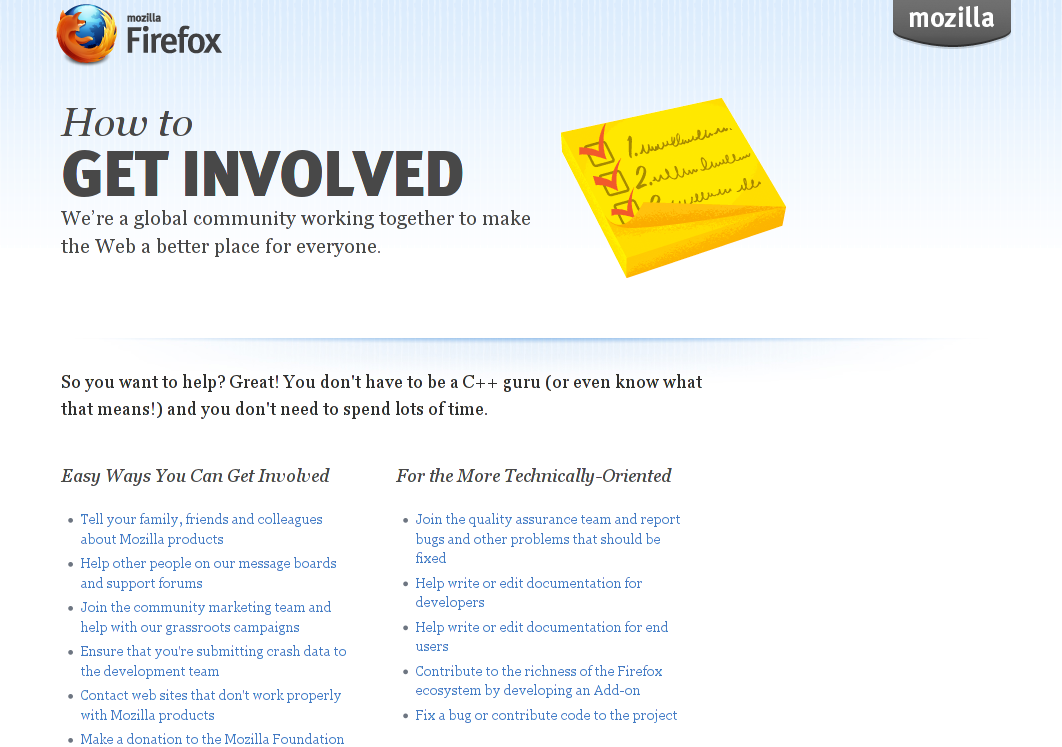
\includegraphics[height=0.8\textheight]{../img/mozilla-get-involved}

    \href{http://www.mozilla.org/en-US/firefox/community/}{http://www.mozilla.org/en-US/firefox/community/}
  \end{center}
\end{frame}

\begin{frame}
  \frametitle{How to Contribute}
  \begin{LARGE} (Sort of) Offline \end{LARGE}
  \begin{itemize}
  \item Summer-of-Codes
    \only<2>{\begin{itemize}
    \item Google SOC
    \item Ruby SOC
    \item New Zealand SOC
    \end{itemize}}
  \item Internships at OS-friendly companies \\ (Red Hat, Mozilla, Untangle, Canonical, etc.)
    % http://www.networkworld.com/news/2008/090208-open-to-watch.html
  \item Local user and developer groups
  \item (Un)Conferences
  \end{itemize}

  \vspace{1em}

  \begin{LARGE} Online \end{LARGE}
  \begin{itemize}
  \item openhatch.org
  \item Software communities: github, Bitbucket, Launchpad, Gitorious, Google Code, SourceForge
  \item Hardware communities: openhardwarehub.com, https://opendesignengine.net/
  \item Content communities: 
  \end{itemize}
\end{frame}

\begin{frame}
  \frametitle{Create}
  \begin{LARGE}
    \begin{tabular}{r l}
      Q: & How does something become open source? \\
      \only<2>{A: & Select a \textcolor{beamer@myblue}{license} and share it with others \\}
    \end{tabular}
  \end{LARGE}

\end{frame}

\begin{frame}
  \frametitle{Software}
  \begin{itemize}
  \item Create your own projects
    \begin{itemize}
    \item Release them under an open source license \\ (GPL, BSD, Apache, etc.)
    \end{itemize}
  \item Contribute to existing projects
  \end{itemize}
\end{frame}

\begin{frame}
  \frametitle{Stuff you should know}
  \begin{overlayarea}{\textwidth}{\textheight}
    \begin{itemize}
    \item Language: whatever the project is written in
    \item Build Process: make, 
    \item Version control: git, CVS, svn, Bazaar, Darcs, Mercurial,
      etc.
    \item Bug Trackers: Bugzilla, Trac, Mantis, Launchpad
    \item Communication: Forums, Wikis, IRC
    \item Source Code Communities: github, Bitbucket, Launchpad,
      Gitorious, Google Code, SourceForge
    \end{itemize}
  \end{overlayarea}

\end{frame}

% http://www.kegel.com/academy/opensource.html
% http://stackoverflow.com/questions/43649/how-to-get-involved-in-an-open-source-project

\begin{frame}
  \frametitle{How to Get Involved}
  \begin{itemize}
  \item Software
    \only<2>{
    \begin{enumerate}
    \item Write software
    \item Release it with an Open Source license
      \begin{itemize}
      \item GNU Public License (GPL): Is now, and will forever be free
      \item BSD License: Is free, but can be used in commercial projects too
      \end{itemize}
    \end{enumerate}}
  \item Hardware
    \only<3>{
    \begin{enumerate}
    \item Build hardware
    \item Make the schematics available to everyone with an open source license
    \end{enumerate}}
  \item Content
    \only<4>{
    \begin{enumerate}
    \item Write, direct, conduct, compose, assemble, cook, generate$\ldots$
    \item Make your work available with a \textcolor{beamer@mygreen}{Creative Commons} License of your choice
      \begin{itemize}
      \item Attribution
      \item Attribution-ShareAlike
      \item Attribution-NoDerivs
      \item Attribution-NonCommercial
      \item Attribution-NonCommercial-ShareAlike
      \item Attribution-NonCommercial-NoDerivs 
      \end{itemize}
    \item Find stuff related to your project to make available
% http://creativecommons.org/choose/
    \end{enumerate}}
  \end{itemize}

  \begin{center}
      \only<2>{
\includegraphics[height=0.2\textheight]{../img/gpl}}
      \only<4>{
\includegraphics[height=0.2\textheight]{../img/creative-commons}}
      \only<5>{
        \begin{Large}
        You can simply add an open license (GPL, Creative Commons, etc.) to something to make it open, just like you can add a \copyright to restrict it and make it "closed."
        \end{Large}}

  \end{center}

\end{frame}

\end{document}
